% Math symbols and examples: http://en.wikibooks.org/wiki/LaTeX/Mathematics
% Also useful link: http://en.wikibooks.org/wiki/LaTeX/Advanced_Mathematics

% This document is used for title generating of exercise solutions. 
% Also it used for generating styles and environmentof documents.
% To add this title in document add next line:
% % This document is used for title generating of exercise solutions. 
% Also it used for generating styles and environmentof documents.
% To add this title in document add next line:
% % This document is used for title generating of exercise solutions. 
% Also it used for generating styles and environmentof documents.
% To add this title in document add next line:
% \input{../template.tex}
\documentclass[a4paper]{article}
\usepackage[utf8]{inputenc}
\usepackage[top=1.5cm]{geometry}
\usepackage{amssymb}
\usepackage{enumitem}
\usepackage{amsmath}

\allowdisplaybreaks

\DeclareMathOperator{\ggT}{ggT}
\DeclareMathOperator{\kgV}{kgV}

\title{Mathematik: Diskrete Strukturen \\ \Large Lösungsblatt}
\author{Anton Bubnov, Eugen Kuzmenko}

\documentclass[a4paper]{article}
\usepackage[utf8]{inputenc}
\usepackage[top=1.5cm]{geometry}
\usepackage{amssymb}
\usepackage{enumitem}
\usepackage{amsmath}

\allowdisplaybreaks

\DeclareMathOperator{\ggT}{ggT}
\DeclareMathOperator{\kgV}{kgV}

\title{Mathematik: Diskrete Strukturen \\ \Large Lösungsblatt}
\author{Anton Bubnov, Eugen Kuzmenko}

\documentclass[a4paper]{article}
\usepackage[utf8]{inputenc}
\usepackage[top=1.5cm]{geometry}
\usepackage{amssymb}
\usepackage{enumitem}
\usepackage{amsmath}

\allowdisplaybreaks

\DeclareMathOperator{\ggT}{ggT}
\DeclareMathOperator{\kgV}{kgV}

\title{Mathematik: Diskrete Strukturen \\ \Large Lösungsblatt}
\author{Anton Bubnov, Eugen Kuzmenko}


\usepackage{wrapfig}
\usepackage{graphicx}
\usepackage{color}

\begin{document}
    \maketitle
    \section*{Vertiefung:}
    \begin{enumerate}[label=(\alph*)]
        % Task (a)
        \item  Ein ebener, $k$-regulärer Graph besteht aus 12 Knoten und teilt die Ebene in 14 Gebiete. 
        Wie groß ist $k$? \\
        Nach Theorem 3.23 gilt $||F|| = ||E|| - ||V|| + 2$. Für unseren Fall bedeutet das also:
        $$14 = ||E|| - 12 + 2 \implies E = 24$$ Des weiteren gilt nach Proposition 3.3:
        $$\sum_{v \in V} deg(v) = 2 \cdot ||E||$$ D.h. die Summe der Grade ist $2 * 24 = 58$.
        Daraus folgt $\frac{58}{12} = 4 = k$
        
        %Task (b)
        \item Gibt es einen ebenen, $k$-regulären Graphen mit 8 Knoten, der die Ebene in 14 Gebiete
        teilt? \\  
        Aus Theorem 3.23 folgt, dass $||F|| = ||E|| - ||V|| + 2$ gilt. Für unseren Fall bedeutet 
        das aus $ 14 = ||E|| - 8 + 2 $ $ ||E|| = 20 $ folgt. Wir haben also einen Graphen mit 8 Knoten 
        und 20 Kanten. Nach Theorem 3.24 gilt für jeden planaren Graphen $ ||E|| \leq 3 \cdot ||V|| - 6$. 
        Für unseren Fall gilt also $20 \leq 3 \cdot 8 - 6  = 18$.
        Wir stoßen auf einen Widerspruch, da $20 \leq 18$ falsch ist. Einen solchen Graphen kann es nicht geben.
        
        %Task (c)
        \item Erweitern Sie die Eulersche Polyederformel auf nichtzusammenhängende, planare Graphen. \\
        Für einen planaren nicht-zusammenhängenden Graphen G mit k Zusammenhangskomponenten beachten 
        wir, dass sich die Komponenten die äußere Fläche gemeinsam teilen. Daraus folgt, dass es im gegensatz 
        zum zusammenhängenden Fall k-1 Flächen weniger gibt. Somit gilt für nicht zusammenhängende Graphen 
        $$||F|| = ||E|| - ||V|| + 2 + (k-1) = ||E|| - ||V|| + 1 + k$$ Für nicht-zusammenhängende Graphen 
        ergibt sich folglich: $$||F|| = ||E|| - ||V|| + 1 + k $$
       
        %Task (d)
        \item Ist der $Q_3$ planar? \\
        Ja. Betrachte dazu folgende Graphik:\\
        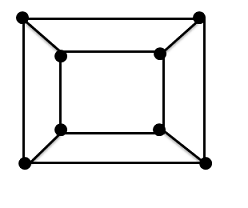
\includegraphics[width=0.3\linewidth]{Q3}
        
        %Task (e)
        \item Ist der $Q_4$ planar?\\
        Nein. Der $Q_4$ enthält einen $K_{3,3}$ als Teilgraphen. Wenn man diesen Teilgraphen ''aufspannt'' 
        gibt es Überkreuzungen im gesamten Graphen. Daraus folgt, dass der $Q_4$ nicht planar sein kann. \\
        Hier der (gut versteckte) $K_{3,3}$ mit den \textcolor{magenta}{direkten Verbindungen} und \textcolor{green}{indirekten Verbindungen} \\ 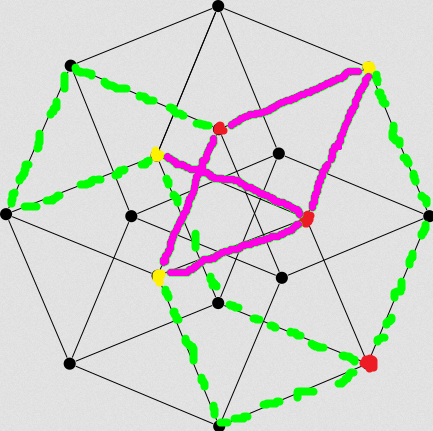
\includegraphics{Q4}
        
        %Task (f)
        \item Es reicht aus die Aussage für kantenmaximale planare Graphen zu zeigen, da hiermit die 
        linke Seite maximiert wird. Sei nun $G=(V,E)$ ein kantenmaximaler und ebener Graph, der keine 
        Dreiecke als Teilgraphen besitzt. Für $||V||=3$ gibt es nur das Äußere und somit nur ein Gebiet. 
        Wenn wir nun einen Knoten hinzufügen, dann müssen wir auch aufgrund der Kantenmaximalität zwei 
        Kanten hinzufügen, wodurch Dreiecke vermieden werden.  Wenn wir dies fortsetzen, erhalten wir:
        $$ 2 \cdot ||F|| \le ||E||\implies 2 \cdot \left(||E|| - ||V|| + 2 \right) \le ||E||$$
        Nach Theorem 3.23 gilt somit:
        $$||E|| \le 2 \cdot ||V|| - 4 $$ 
        
        % Task (g)
        \item Besitzt jeder planare, dreiecksfreie Graph einen Knoten $v$ mit $deg(v) \leq 3$? \\
        Wir führen einen Beweis durch Widerspruch: Angenommen es gibt einen planaren, dreiecksfreien Graphen mit der Eigenschaft, dass bei jedem Knoten der Grad strikt größer als drei ist. Dann gilt: 
        \begin{align*}
            4 \cdot ||V|| &\geq \sum_{v \in V} deg(v)
            &= 2 \cdot ||E|| (Proposition 3.3)
            &\geq 4 \cdot ||V|| - 8 (Vertiefung f)
        \end{align*}
        Wir erhalten einen Widerspruch. Also besitzt jeder planare Graph einen Knoten mit der Eigenschaft $deg(v) \leq 3$
        % Task (h)
        \item Kein Antwort

        % Task (i)
        \item Wie viele Knotenfärbungen mit k Farben hat ein $K_n$? \\
        Da jeder Knoten n-1 Nachbarn hat (jeder Knoten ist mit jedem verbunden) hat der $K_n$ $n$ Farben. 
        Der erste Knoten kann beliebig gewählt werden, weshalb es $k$ Möglichkeiten zur Färbung gibt. 
        Für die weiteren Knoten gibt es immer eine Möglichkeit weniger, für eine Färbung. Folglich gibt es: \\
        $\prod_{i=0}^{k-1} k - i = k^{\underline{n}}$ Möglichkeiten zur Färbung eines $K_n$.
          
        % Task (j)
        \item Wie ist die chromatische Zahl eines $Q_d$? \\
        Für den Sonderfall $d = 1$ reicht eine Farbe aus. \\
        Für den Fall $d = 2$ haben wir zwei Knoten, die über einen Graph mit zwei Knoten die über eine Kante verbunden sind. Hier ist die chromatische Zahl trivialer Weise 2.\\
        Für $d \geq 3$ betrachten wir die Definition des Hyperwürfels. Nach der Definition des Hyperwürfels gilt, dass der $Q_d$ immer quadratische Flächen hat bzw. Kreise der Länge 4. Da man für einen   Kreis mit gerader Knotenanzahl mit minimal zwei Farben für eine Knotenfärbung auskommt, gibt es auch einen $Q_d$ der mit nur zwei Farben auskommt, wenn man den Kreis mit vier Knoten und Kanten ''ausdimensionalisiert'' und den jeweils neu entstehenden ''Ecken'' eine andere Farbe zuteilt als dem entsprechenden Nachbarknoten aus der ''vorherigen Dimension''. Die chromatische Zahl des $Q_d$ für $d \geq 2$ ist somit 2.
        
    \end{enumerate}
    \section*{Kreativität:} Wie viele Knotenfärbungen mit 3 Farben hat der Kreis $C_n$ ?\\
    Hinweis: Stellen Sie eine geeignete Rekursionsgleichung auf und lösen Sie diese.\\
    \\
    Wenn wir anfangen den Kreis mit unseren 3 Farben zu färben, dann können wir bei einem beliebigen Knoten unseren Anfang setzen. Wir denken uns nun eine der beiden Kanten vom Anfangsknoten weg und erhalten einen zusammenhängenden Graphen mit der Eigenschaft $||E|| = n-1$, also einen Baum. Um den Anfangsknoten zu färben stehen 3 Möglichkeiten zur Verfügung, wodurch sich 3 verschieden gefärbte Binärbäume konstruieren lassen, die aber alle die gleiche Struktur haben (es entstehen verschiedene Binärbäume da die Wurzelfarbe jeweils unterschiedlich ist). Zur Visualisierung zeigt die eingefügte Graphik den konstruierten Binärbaum bis hin zum $C_6$ für den Fall, dass man dem ersten Knoten die Farbe 1 zugeordnet hat. Offensichtlich gibt es im Kreisgraphen bis zum Vorletzten Knoten 2 Möglichkeiten zur weiteren Färbung. Wir halten im Binärbaum mit jeden weiteren Blättern die "Färbungspfade" fest. 
        \begin{wrapfigure}{l}{0.25\textwidth}
            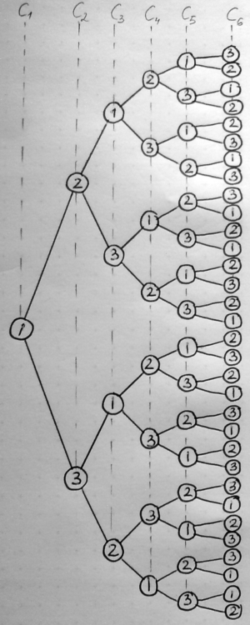
\includegraphics[width=1\linewidth]{baum_kreativ}
        \end{wrapfigure}\\
     Wir können sehen, dass die eingefügte Graphik alle Variationen für einen $C_1$ bis hin zum $C_6$  wiedergibt. \\
     Wir müssen allerdings beachten, dass wir manche Knoten ''zu oft abzählen'', da sie nicht in das Färbungsschema hineinpassen. In unserer Graphik sind das beispielsweise für den $C_6$  immer die Knoten, die die Farbe 1 haben. Wir müssen folglich für jeden der drei Bäume  mit den verschiedenen Wurzelfärbungen stets die Anzahl an Knoten abziehen, die eine Farbe erhalten würden, die mit der Farbe der Baumwurzel übereinstimmt.\\
     Für den Binärbaum, mit der Baumwurzel, die die Farbe 1 erhalten hat, ist die gesamte Anzahl der Knoten $2^n-1$. Wir färben nun jedes Blatt mit jeweils einer anderen Farbe wir die Wurzel gefärbt haben. Für alle weiteren Blätter bzw. Subbäume wenden wir das gleiche Färbungsschema an und erhalten somit einen Baum mit $2^n-1$ Färbungen. Da wir den ersten Knoten (die Baumwurzel) auch mit der 2 oder 3 Färben können, lassen sich analog 2 weitere Binärbäume aufspannen, die das gleiche Schema besitzen, aber weitere Möglichkeiten zur Färbung, die uns fehlen, wenn wir die Wurzel mit der 1 färben. Wir halten eine ''Gesamtfarbenbelegungsanzahlanzahl'' mit $3\cdot 2^{n-1}$ Möglichkeiten (vorerst) fest. Dies ist gerade die Anzahl der Knoten in den untersten Baumebenen.
     Von dieser müssen wir nun die Anzahl der gefärbten Knoten abziehen, die uns nicht passen. Dies sind gerade diejenigen Knoten in der untersten Baumebene, deren Farbe mit der Farbe der Baumwurzel übereinstimmt. Die Anzahl dieser Knoten erhalten wir stets, indem wir uns die Möglichkeiten für die Färbung in der "Baumebene darüber" berechnen.
     
     Somit können wir folgende rekursive Formel aufstellen, die die Anzahl der Knotenfärbungen 
     berechnet. Für den $C_0$  und $C_1$ gibt es keine Möglichkeiten, denn ein Kreis muss aus mindestens 3 Knoten bestehen. Für die Gültigkeit unserer rekursiven Formel fassen wir fassen einen Pfad aus zwei Knoten und einer Kante als Sonderfall eines Kreises auf ( der 6 mögliche Färbungen besitzen kann) und für den $C_n$ gelte somit: 
     \begin{align*} 
     a_0 &= 0 \\ 
     a_1 &= 0  \\
     a_n &= 3\cdot 2^{n-1} - a_{n-1}\\ 
     \end{align*}
     Nun wollen wir unsere rekursive Formel in eine explizite (nicht-rekursive) Form überführen. Wir schreiben die ersten 5 Knotenfärbungen auf:
     \begin{align*}
          a_0 &= 0\\
          a_1 &= 0\\
          a_2 &= 3\cdot 2^1 - a_1 = 3\cdot 2^1\\
          a_3 &= 3\cdot 2^2 - a_2 = 3\cdot 2^2 - 3\cdot 2^1\\
          a_4 &= 3\cdot 2^3 - a_3 = 3\cdot 2^3 - (3\cdot 2^2 - 3\cdot 2^1)\\
          a_5 &= 3\cdot 2^4 - a_4 = 3\cdot 2^4 - (3\cdot 2^3 - (3\cdot 2^2 - 3\cdot 2^1))\\
          &= 3\cdot 2^4 - 3\cdot 2^3 + 3\cdot 2^2 - 3\cdot 2^1\\
          &= 3\cdot (2^4 - 2^3 + 2^2 - 2^1)
        \end{align*} 
     Ohne Beeinträchtigung der Allgemeinheit können wir folglich unsere rekursive Formel wie folgt überschreiben:
     $$ a_n = 3 \cdot (-1)^{n-1} \cdot \sum_{k=1}^{n-1}(-2)^k$$
    \section*{Transfer:}
    \begin{enumerate}[label=(\alph*)]
    	\item Wie viele Kanten benötigen Sie für einen (n, d)-dimensionalen De Bruijn-Graphen?\\
        Im ungerichteten Graphen können wir ab mehr als einen Knoten, 3 verschiedene Gruppen von Knoten, die sich in ihren Knotengraden unterscheiden, festlegen. Die erste Gruppe dieser Knoten ist in der Form $(x,x,x,\ldots)$ mit $x \in [d]$ und für diese Gruppe gilt $\textrm{deg}(v) = 2d -2$. Die 2. Gruppe der Knoten hat die Form $(x,y,x,y,\ldots)$ mit $x \not = y$ und $x,y \in [d]$, für diese Gruppe gilt $\textrm{deg}(v) = 2d -1$. Zu guter Letzt gibt es noch die letzte Gruppe, die aus den restlichen Knoten besteht, die nicht die Form der bereits vorherigen Gruppen besitzen. Für solche Knoten gilt $\textrm{deg}(v) = 2d$.\par
        In Gruppe 1. befinden sich $d$ Knoten, in Gruppe 2. $d^2-d$ Knoten und in Gruppe 3. $d^n - d - d(d-1)$ Knoten. Benutzt man nun Proposition 3.3, so erhält man die Anzahl der Kanten. 
        \begin{align*}
        d(2d-2) + (d^2-d)(2d-1) + 2d(d^n-d-d(d-1)) &= 2d^{n+1}-d^2-d
        \end{align*}
        
        Durch Anwendung von Proposition 3.3 erhalten wir:
        \begin{align*}
        ||E|| = \frac{2d^{n+1}-d^2-d}{2}
        \end{align*}
        
        \item In einem solchen Graphen beträgt der maximale Abstand zweier Knoten $n$
        
        \item Wir suchen uns ein Tupel der Form $(1,\ldots,1)$ und bezeichnen ihn als $x_1$. Von diesem aus betrachten wir alle Verbindungen zu all anderen Knoten, welche maximal $n$ entfernt liegen (Teilaufgabe (b)). Nun verfahren wir wie folgt: \par
        Wir gehen von einem beliebigen Knoten rückwärts zu dem Knoten $x_1$ zurück  und summieren dabei die Zahlenwerte auf. Dabei werden jeweils 3 Rechenschritte benötigt (Lesen, Addition, Schreiben). Nun kann es passieren, dass Zahlenwerte doppelt gezählt werden, um dies zu vermeiden muss man nochmal über die Knoten iterieren und alles mit 0 überschreiben. Nun suchen wir uns solange einen Knoten aus, der keine 0 stehen hat und wiederholen das Prozedere solange, bis kein solcher Knoten mehr existiert. \par
        Somit erhält man für die Anzahl der Rechenschritte $(nd^n-2n)(3nd^n-3n)$.
    \end{enumerate}
\end{document}